% Drawing 136/05-1 -- folder 136, batch 05, archive page 90 (PDF page 91).
% Transcription: à gauche, un schéma à traits sans flèches\,: $k$ relié par $u$, $u'$, $u''$ à $\Phi$, $\Phi'$ (écrit deux fois, un tracé biffé), $\Phi''$\,; $\Phi,\Phi'$ vers $N$, $\Phi',\Phi''$ vers $N'$, puis $N$ et $N'$ vers $N''$
% Kind: diagram of strokes without arrows. Method 2 (schematic redraw from the facsimile). Status: ok.
% Notes: k joined by u, u', u'' to Phi, the first Phi', Phi''; Phi and the first Phi' to N, the second Phi' and Phi'' to N'; N and N' to N''. Omitted as struck: the stroke from k to the second Phi' (scribbled over on the page), so the second Phi' has no stroke from k. The small u labels are tiny and placed by eye. Issue 128, 2026-11-09: struck material left out after a fresh check of the facsimile (struck-out material is not drawn). Redrawn 2026-11-09 (issue 128): to check again. Question settled by a machine pass on the facsimile, 2026-11-12 (maths): the first Phi' already carries the stroke u' from k, and the second Phi' is the same object written again for N', so leaving out the struck stroke loses no relation; the drawing stays as it is. Not checked by a reader.
% Coordinates: 1 unit = 1 mm = 1/100 of the crop width (bbox in page fractions: [0.08, 0.06, 0.5, 0.2]).
% Redrawn by Claude (claude-opus-5-5), issue #73, 2026-11-07; not checked by a human; not compiled (no TeX in the session).
% Rights: reproduces part of the work -- behind RENDER_TRANSCRIPTS, never published by itself.
\documentclass[tikz,border=3pt]{standalone}
\usepackage{amsmath,amssymb}
\usetikzlibrary{patterns,arrows.meta}
\tikzset{pencil/.style={black!45}, struck/.style={black!35}, mark/.style={circle,draw,inner sep=1.3pt}, pt/.style={circle,fill,inner sep=0.9pt}, opt/.style={circle,draw,fill=white,inner sep=1.1pt}}
\begin{document}
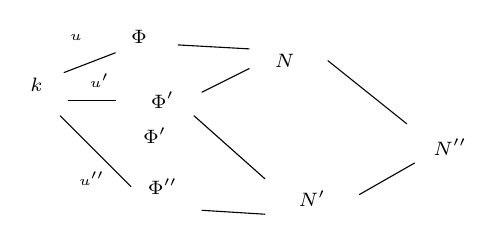
\begin{tikzpicture}[x=1mm,y=1mm,line cap=round,line join=round,font=\scriptsize]
\node[inner sep=1pt] at (28,-22) {\scriptsize $k$};
\node[inner sep=1pt] at (41,-16) {\scriptsize $\Phi$};
\node[inner sep=1pt] at (44,-24) {\scriptsize $\Phi'$};
\node[inner sep=1pt] at (43,-28.5) {\scriptsize $\Phi'$};
\node[inner sep=1pt] at (44,-35) {\scriptsize $\Phi''$};
\node[inner sep=1pt] at (59.5,-19) {\scriptsize $N$};
\node[inner sep=1pt] at (63,-36.5) {\scriptsize $N'$};
\node[inner sep=1pt] at (80.5,-30) {\scriptsize $N''$};
\draw (31.5,-20.5) -- (38,-18);
\draw (32,-24) -- (38,-24);
\draw (31,-26) -- (40,-35);
\node[inner sep=1pt] at (33,-16) {\tiny $u$};
\node[inner sep=1pt] at (36,-21.5) {\tiny $u'$};
\node[inner sep=1pt] at (35,-34) {\tiny $u''$};
\draw (46,-17) -- (55,-17.5);
\draw (49,-23) -- (55,-20);
\draw (48,-26) -- (57,-34);
\draw (49,-38) -- (57,-38.5);
\draw (65,-19) -- (75,-27);
\draw (69,-36) -- (76,-32);
\end{tikzpicture}
\end{document}
